\documentclass{homework}
\usepackage{lipsum}
\usepackage{cancel}
\usepackage{amsthm}
\usepackage{cleveref}
\usepackage{upgreek}
\usepackage{mathrsfs}
\usepackage{tikz}
\usepackage{units}
\newtheorem{lemma}{Lemma}

\DeclareMathOperator{\cov}{cov}

\title{Kevin Joyce}
\course{Stat 542 - Applied Linear Models - Test 1}
\author{Kevin Joyce}
\docdate{\today}
\begin{document} 
\newcommand{\figref}[1]{\figurename~\ref{#1}}
\renewcommand{\bar}{\overline}
\renewcommand{\hat}{\widehat}
\renewcommand{\SS}{\mathcal S}
\newcommand{\HH}{\mathscr H}
\newcommand{\mom}{\widetilde}
\newcommand{\mle}{\widehat \Uptheta}
\newcommand{\eps}{\varepsilon}
\newcommand{\todist}{\stackrel{D}\longrightarrow}
\newcommand{\toprob}{\stackrel{p}\longrightarrow}
\newcommand{\TTheta}{\overline{\underline \Theta} }
\newcommand{\del}{\partial}
\newcommand{\approxsim}{\overset{\cdotp}{\underset{\cdotp}{\sim}}}
\newcommand{\RSS}{\ensuremath{\mathrm{RSS}}}
\newcommand{\MSE}{\ensuremath{\mathrm{MSE}}}
\newcommand{\SE}{\ensuremath{\mathrm{SE}}}
\newcommand{\TSS}{\ensuremath{\mathrm{TSS}}}
\newcommand{\SSReg}{\ensuremath{\mathrm{SSReg}}}
\begin{longproblem}
The rise in abundance of algae in coastal waters is thought to be due to increase
in nutrients such as nitrates and other forms of nitrogen.  It is theorized
that the excessive amounts of nitrate are due to human influences.  Human
populations can affect nitrogen inputs to rivers through industrial and
automobile emissions to the atmosphere (causing the nitrogen to enter the river
through rainfall), through fertilizer runnoff, through sewage discharge, and
through watershed disturbance.  Researchers gathered data from 42 rivers around
the world to gauge the evidence that nitrates in the discharges of rivers
around the world are associated with human population density. The data are on
the course webpage under the filename \texttt{nitriver.txt}.  Among the
variables measured were:
\begin{align*}
  y   = &\text{ nitrate concentration (\unit{$\mu$M/l})}\\
  x_1 = &\text{ discharge: the estimated annual average discharge of the river into the ocean 
  ($\mathrm l/\mathrm{sec} \times \mathrm k \times \mathrm m^2$) }\\
  x_2 = &\text{ runoff: the estimated annual average runoff from the watershed ($\mathrm l/\mathrm{sec} \times \mathrm k \times \mathrm m^2$) }\\
  x_3 = &\text{ precipitation (cm/year) }\\
  x_4 = &\text{ area of watershed ($\mathrm{km^2}$) }\\
  x_5 = &\text{ human population density } (\mathrm{people}/\mathrm{km}^2)\\
  x_6 = &\text{ deposition: the product of precipitation times nitrate concentration}\\
  x_7 = &\text{ nitrate precipitation:  the concentration of nitrate in wet precipitation at sites }\\
       &\text{ located near the watersheds }(\mu\mathrm{mol}\,\mathrm{NO}_3/(\mathrm{sec}\times\mathrm{km}^2)\\
  x_8 = &\text{ nitrate export: the product runoff times nitrate concentration. }\\
\end{align*}

  \subproblem{ Perform some exploratory data analysis on these variables and
  write a brief (no more than 2 paragraphs) summary of your findings.  Since
  nitrate concentration is the response variable, your analysis should focus on
  the relationship between nitrate concentration and the other variables, as
  well as any relationships among the explanatory variables.  Also include in
  your discussion what problems you might expect to encountering trying to
  determine a best model according to some selection criterion.  [Do NOT
  actually look for a ``best'' model - I am just looking for what problem(s)
  you might anticipate in the process of finding such a model based on your
  EDA.]}
  \begin{solution}
  Each variable is quantitative, hence, comparisons can be made with scatter
  plots between each variable.  The histograms in the following plot indicate
  that each variable is right skewed to varying degrees.  There is a data point 
  (index 34) that has very large \texttt{nitconc}, \texttt{discharge} and
  \texttt{runoff} indicating a potential outlier. 

  In the comparisons with \texttt{nitconc}, it appears that discharge, run-off,
  precipitation, and area are weakly, if at all, correlated with the response.
  Population density, deposition, nitrate precipitation, and nitrate export
  are moderately correlated (positively) with nitrate concentration.  The
  linearity of the relationships are not perfect, and a transformation (perhaps
  log-log due to each being right skewed) may be appropriate.  Additionally,
  there may be collinearity issues among density, deposition, nitrate
  precipitation, and nitrate export, and also among discharge, runoff,
  precipitation, and area due to their apparent correlation (although discharge
  and runoff do not appear to be correlated). 

  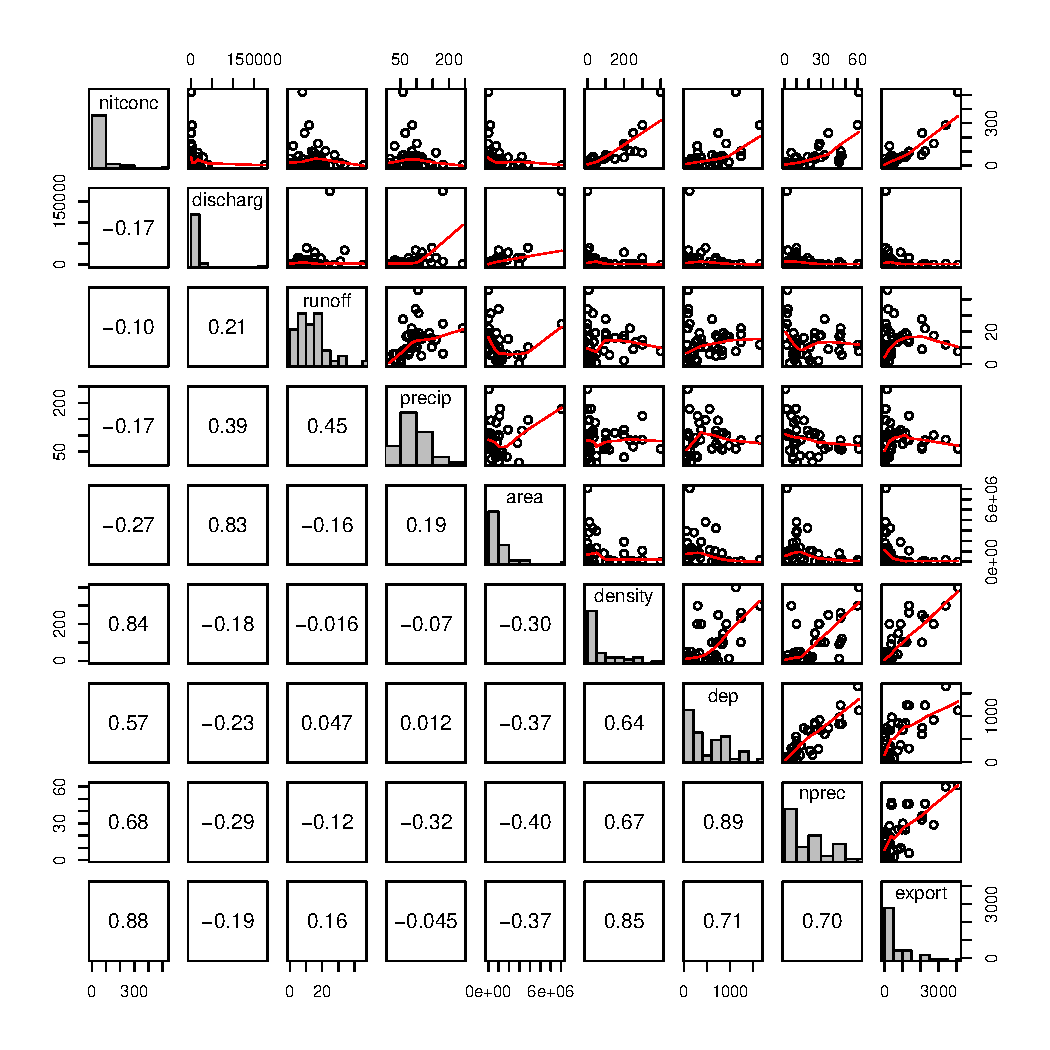
\includegraphics[width=.9\textwidth]{eda_problem1.pdf}
  \end{solution}

  \subproblem{ Suppose after examining the numerous models, you decide that the general linear model with explanatory variables $(x_2,x_6,x_7,x_8)$ is the best model.  Using the ``best'' model, give a set of Bonferroni joint confidence intervals for the model parameters.  Explain in a sentence or two why it is important to use a Bonferroni correction here. }
\begin{solution}
  The 95\% Bonferroni corrected confidence intervals are given in the following table:

  \begin{center}
  \begin{tabular}{l r l}
  \hline
  $\hat\beta_0\pm t_{1-.05/(2\cdot5)}(n-5)\cdot\SE(\beta_0)=$ & $25.198 \pm 35.592$ &\text{ or }$(-10.394, 60.790)$ \\
  $\hat\beta_2\pm t_{1-.05/(2\cdot5)}(n-5)\cdot\SE(\beta_2)=$ & $-1.850 \pm  1.774$ &\text{ or }$( -3.625, -0.076)$ \\
  $\hat\beta_6\pm t_{1-.05/(2\cdot5)}(n-5)\cdot\SE(\beta_6)=$ & $-0.094 \pm  0.088$ &\text{ or }$( -0.182, -0.007)$ \\
  $\hat\beta_7\pm t_{1-.05/(2\cdot5)}(n-5)\cdot\SE(\beta_7)=$ & $ 2.077 \pm  2.226$ &\text{ or }$( -0.149,  4.302)$ \\
  $\hat\beta_8\pm t_{1-.05/(2\cdot5)}(n-5)\cdot\SE(\beta_8)=$ & $ 0.091 \pm  0.024$ &\text{ or }$(  0.067,  0.115)$ \\\hline
  \end{tabular}
  \end{center}

  Since there is joint uncertainty in estimating
  $(\beta_0,\beta_2,\beta_6,\beta_7,\beta_8)$ simultaneously, the Bonferroni
  correction protects against falsely rejecting one of the tests
  $H_0:\,\beta_k=0,\,k=0,2,6,7,8$. That is, this protects against Type I errors.
\end{solution}

  \subproblem{ In the ``best'' model of part (b), perform a permutation test of $H_0\,:\,\beta_7 =0$ where $\beta_7$ is the parameter corresponding to $x_7$.  Report the permutation p-value and a clear conclusion to the test.  Does this agree with the normal-based p-value reported in the \textbf{Coefficients} table?}

\begin{solution}
  We fit the ``best'' model with 4999 permutations of the \texttt{nprec}
  variable and compare the computed $F$-statistic for significance of $\beta_7$
  between the permuted and un-permuted model. The ratio of the number of those where the
  permuted model resulted in a more significant statistic and the total number of permutations (counting the original ordering) was found to be $p = (67+1)/(4999+1) = 0.0136$.  This is comparable with the $p$-value (0.0156) given by the normal based test.
\end{solution}
\end{longproblem}

\begin{longproblem}
  As part of a study of the effects of predatory intertidal crab species on snail populations, researchers measured the mean closing forces and the propodus heights of the claws on several crabs of three species. Specifically, there were three crab species in the study (\emph{Hemigrapsus nudus, Lophopanopeus bellus, Cancer productus}) with between 12-14 crabs of each type on which measurements were taken.  The data are given below and can be found on the course webpage under the filename \texttt{crab.txt}.

  Let:
  \begin{align*}
    y   &=\quad \text{the log mean closing force of a crab,}\\
    x_1 &=\quad \text{the log mean propodus height of a crab claw,}\\
    x_2 &=\quad \begin{cases} 1&\text{if the crab species is \emph{H. nudus}}\\ 0 & \text{otherwise}\end{cases}\\
    x_3 &=\quad \begin{cases} 1&\text{if the crab species is \emph{L. bellus}}\\ 0 & \text{otherwise.}\end{cases}\\
  \end{align*}

  \subproblem{Consider the multiple linear regression model given by:
  $$
    y_i = \beta_0 +\beta_1x_{i1} +\beta_2x_{i2}+\beta_3x_{i3}+\beta_4x_{i1}x_{i2} + \beta_5x_{i1}x_{i3} + \epsilon_i.
  $$
  Interpret the parameters $\beta_1,\beta_2,\&\beta_4$ clearly \emph{in the context of the problem}. For example, do not just say: ``$\beta_1$ is the partial slope of $y$ on $x_1$.''  Explain its meaning in terms of the mean respons $y$. }
  \begin{solution}
    Throughout this analysis, we use base 10 logarithms.
    For each $i$th response, there are three cases for
    $(x_{i2},x_{i3})$: $(x_{i2},x_{i3}) = (0,0)$, in which case the
    species is species \emph{C. productus}; $(x_{i2},x_{i3})=(0,1)$,
    in which case the species is \emph{L. bellus}; or
    $(x_{i2},x_{i3})=(1,0)$, and the species is \emph{H. nudus}.
    
    When  $(x_{i2},x_{i3})=(0,0)$, $y_i = \beta_0 + \beta_1x_{i1} +
    \epsilon_i$, whose expected value transformed back is $10^{\beta_0+ \beta_1
    x_{i1}}$.  From this we see that $\beta_0$ is the (not so informative)
    order of 10 when the propodus height is 1.  The interpretation of
    $\beta_1$ is for a 10-fold increase in propodus height, we expect
    $\beta_1$ 10-fold increases in mean closing force. 
    
    
    When $(x_{i2},x_{i3}) =
    (0,1)$, $y_i = (\beta_0+\beta_3) +(\beta_1+\beta_5)x_{i1} +
    \epsilon_i$, and we see that $\beta_3$ is the increase in the
    intercept for the log model when switching from \emph{C. productus} to \emph{L.
    bellus} and $\beta_5$ is the increase in the effect of log propodus
    height on log force.  Similarly when $(x_{i2},x_{i3}) = (0,1)$,
    $y_i = (\beta_0+\beta_2) +(\beta_1+\beta_4)x_{i1} + \epsilon_i$,
    and $\beta_2$ is the increase in the intercept when \emph{C.
    productus} switches to \emph{H. nudus}, and $\beta_4$ is the
    increase in the effect of the log height on the log force for a similar
    species change.
    \end{solution}

  \subproblem{ Construct a scatterplot of log force vs. log height, with a different symbol for each crab species.  In a few sentences, describe the associations between the three variables (log force, log height, crab species). }
  \begin{solution}
  \begin{minipage}{.5\textwidth}
  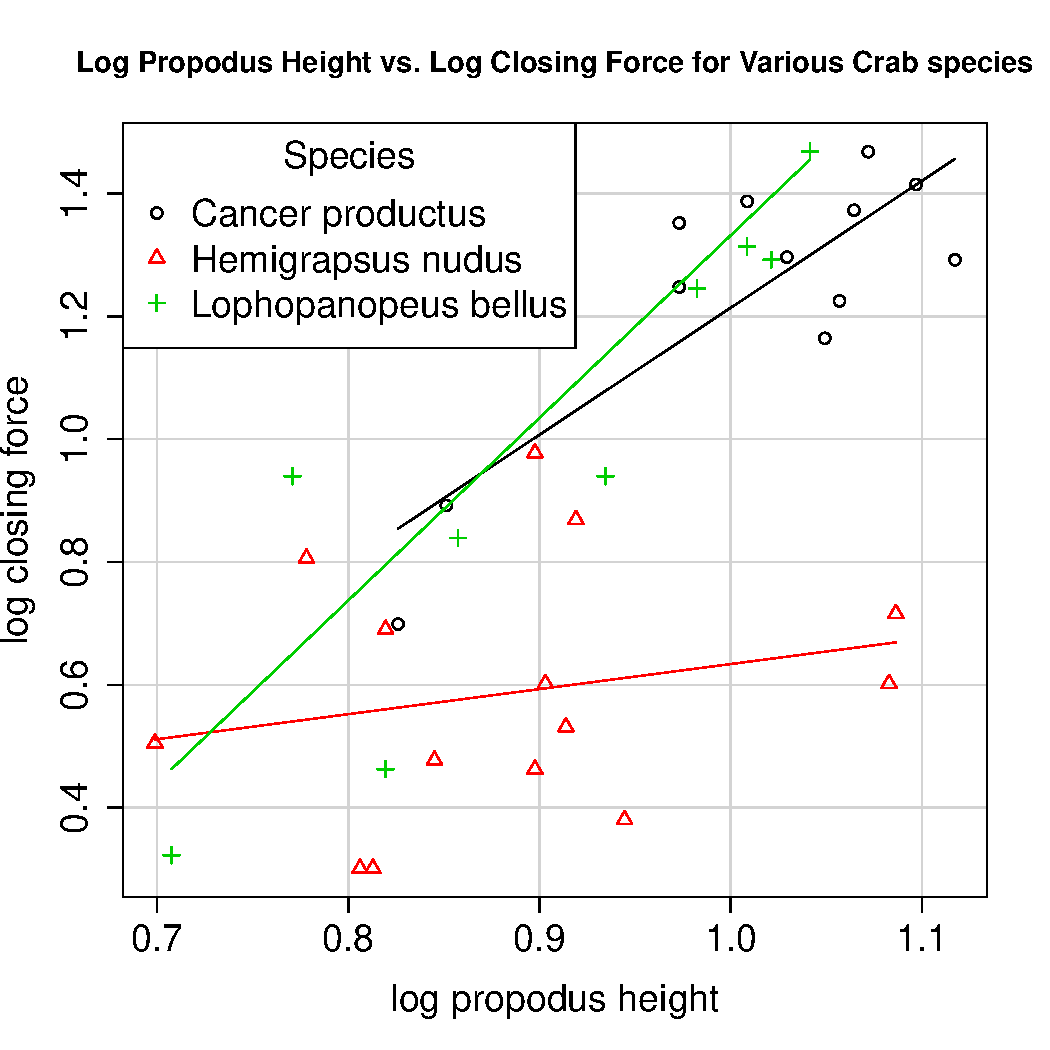
\includegraphics[width=\textwidth]{crab_scatter.pdf}
  \end{minipage}
  \begin{minipage}{.5\textwidth}
  Each species has a positive association between log force and log
  height.  There appears to be an effect of species on this
  association as the slope of \emph{H. nudus} appears to be less
  than those for \emph{C. propodus} and \emph{L. bellus}.  Moreover, the average force appears to be less overall for \emph{H. nudus} than both \emph{C. productus} and \emph{L. bellus}.
  \end{minipage}
  \end{solution}
  
  \subproblem{ Fit the multiple linear regression model $y_i = \beta_0 +\beta_1x_{i1} +\beta_2x_{i2}+\beta_3x_{i3}+\beta_4x_{i1}x_{i2} + \beta_5x_{i1}x_{i3} + \epsilon_i$.  Report the \textbf{ANOVA} and \textbf{Coefficients} table. Test simultaneously whether or not either of the interactions are significant. [As always, give the hypotheses, test statistic, p-value, and a clear conclusion based on this p-value.] Do the results of this test confirm or refute what is seen in the scatter plot? Explain.}
  \begin{solution}
{\small
\begin{minipage}{.50\textwidth}
\begin{tabular}{c c c c c}
\multicolumn{5}{c}{\bf Coefficients Table} \\ \hline
Predictor & $\hat \beta_k$ & $\mathrm{SE}(\hat \beta_k)$ & $t$ & p-val \\ \hline
Intercept & -0.8544  & 0.6293  & -1.358  & 0.18405   \\
$x_1$     &  2.0685  & 0.6208  &  3.332  & 0.00219   \\ 
$x_2$     &  1.0798  & 0.7646  &  1.412  & 0.16752   \\
$x_3$     & -0.7873  & 0.8049  & -0.978  & 0.33536   \\
$x_1x_2$  & -1.6601  & 0.7889  & -2.104  & 0.04330   \\
$x_1x_3$  &  0.9052  & 0.8302  &  1.090  & 0.28368   \\\hline
\end{tabular}
\end{minipage}
\begin{minipage}{.4 \textwidth} 
\begin{center}
\begin{tabular}{c c c c c c}
\multicolumn{6}{c}{\bf Analysis of Variance Table}\\
\hline
Source     & df     & SS        & MS        & F        & p-val   \\ \hline
Regression & 5      & 4.3740    & 0.875     & 24.75    &3.94e-10 \\
Error      & 32     & 1.1311    & 0.0353    &          &         \\
Total      & 37     & 5.5054    & 0.149     &          &         \\ \hline
\end{tabular}
\end{center}
\end{minipage}
}

We test $\beta_4=\beta_5=0$ by computing
$$
  F = \frac{R(\beta_4,\beta_5|\beta_0,\dots,\beta_3)}{\MSE} \approx \frac{0.4497}{0.0353} \approx 6.36,
$$
for which $p < .005$.  Hence, there is significant evidence for both
  interaction effects in the model; i.e. the increase in mean closing force due
  to log propodus height depends on the species.  This agrees with the
  qualitative analysis in the last part since we observed that \emph{not} all
  slopes are the same.
\end{solution}

  \subproblem{ Predict the mean closing force using a 95\% prediction interval for a crab of species \emph{L. bellus} with a propodus height of 11.5.  Would you expect the prediction interval to be wider or narrower if the height had been 8? Explain in a sentence or two.}
\begin{solution}
  We are predicting for the vector $\vect{x_0}' = (1,\log 11.5, 0, 1, 0, \log 11.5)$, so the 95\% prediction interval for the \emph{log} mean closing force is given by
\begin{align*}
  \vect{x_0}'\vect{\hat\beta} \pm t_{.975}(n-p)\cdot&\sqrt{\MSE\cdot (1 + \vect{x_0}'(\vect{X'X})^{-1}\vect {x_0})} \\
  &\approx 1.513 \pm 0.435 \\&\text{ or }( 1.077, 1.948 ).
\end{align*}
Transforming back to mean force, we have
$$
  32.55 \pm 2.72\text{ or }( 29.823, 35.27 ).
$$
The correpsonding interval for $8$ would be narrower for two reasons: first, the inflation due to the reverse transformation $10^x$ would be less, and second, $\log 8\approx 0.94$ is closer to the mean log force value ($\approx .90$) than $\log 11.5 \approx 1.06$.  In fact, if we look at the scatterplot in (b), we see that $\log 11.5$ is larger than any \emph{L. bellus} observation, hence the width will be wider than any observation within the range of \emph{L. bellus} data.
\end{solution}

  \subproblem{ Still considering the full model, test for a difference in the slopes between log force and log height for the \emph{H. nudus} and \emph{C. productus} crab species.  That is, test whether or not the slopes resulting from a regression of log force on log height are different for the two crab species. }
\begin{solution}
  As per the interpretation in part (a), this amounts to testing the significance of the second interaction term; $H_0:\,\beta_4=0$. From the coefficients table, the $t$-test for $t=-2.1$ gives $p=0.043$ and suggests a possible difference from zero.  So there is some evidence for differing associations between mean closing force and height between \emph{H. nudus} and \emph{C. productus}
\end{solution}

  \subproblem{ Another way we might test for difference in the slopes of the regression lines between log force and log height for the three crab species is to run separate regression for the three species, and compare the slopes using 3 independent t-tests.  Discuss in a short paragraph which of these two methods (3 independent t-test, multiple regression) would be better and why?  Think about degrees of freedom, and the mean squared error. [Do NOT perform the tests to answer this question.]}
\begin{solution}
  The two sample $t$-test comparing the normally distributed coefficients
  indicated would test a $t$-statistic with $n_1+n_2-2$ degrees of freedom
  ($n_i$ depending on which populations are in consideration), where the tests
  in multiple linear regression on the same hypothesis (either $\beta_4 = 0$ or
  $\beta_5=0$) would have $n-5$ degrees of freedom.  For these sample sizes,
  the $t$-statistics for multiple linear regression will have more degrees of
  freedom than the ones for the pairwise comparisons.   Moreover, in each case
  to calculate the $t$-statistics, we divide by standard errors for the
  estimates we are testing.  In the multiple linear regression case, the
  squared standard error has $n-5$ in the denominator and the pair-wise tests
  will have $n_1+n_2-2$ in the denominator.  Assuming that the algebra for the
  numerators yields numbers on the same order ($(\vect{X'X})^{-1}_{ii}$ in the
  first case and $(n_1-1)s^2_1 + (n_2-1)s^2_2$ in the other), we would expect
  the standard error for multiple linear regression to be less.  Both of these
  factors (more dfs and smaller standard error) makes the multiple linear
  regression method a more powerful test for finding significance. 
\end{solution}
\end{longproblem}


\begin{longproblem}
  A study was undertaken in major US cities to examine the effects of pollution levels on mortality, adjusting for climate and socioeconomic information.  Specifically, data were collected at each city on the following variables:
\begin{align*}
  y   = &\text{ mortality rate (deaths per 100,000 people over a 3-year period), }\\
  x_1 = &\text{ \texttt{precip} = mean annual precipitation (inches) }\\
  x_2 = &\text{ \texttt{education} = the mean number of school years completed, for persons of age 25 years or older, }\\
  x_3 = &\text{ \texttt{nonwhite} = the percentage of the population that is non-white, }\\
  x_4 = &\text{ \texttt{NOx} = the relative pollution potential of oxides and nitrogen, }\\
  x_5 = &\text{ \texttt{SO2} = the relative pollution potential of sulfer dioxide. }\\
\end{align*}

The primary goal of the study was to investigate whether or not mortality is associated with either of the two pollution variables after accounting for the effects of the climate and socioeconomic variables on mortality.  Suppose a sequence of models was fit with this in mind, resulting in the output tables given below.

{\small
\renewcommand{\a}[1]{{\color{red} \it #1}}
\begin{minipage}{.50\textwidth}
\begin{tabular}{c c c c c}
\multicolumn{5}{c}{\bf Coefficients Table} \\ \hline
Predictor & $\hat \beta_k$ & $\mathrm{SE}(\hat \beta_k)$ & $t$ & p-val \\ \hline
Intercept & 1000.1021 & 92.3981  & \a{10.824} & 3.85e-15   \\
$x_1$     & 1.3792    & 0.7000   & \a{1.970 } & 0.053943   \\ 
$x_2$     & -15.0790  & 7.0706   & \a{-2.133} & 0.037519   \\
$x_3$     & 3.1602    &\a{0.6287}&    5.026   & 5.84e-06   \\
$x_4$     & -0.1076   & 0.1359   & \a{-0.792} & 0.432066   \\ 
$x_5$     &\a{0.3555} & 0.0914   & \a{3.889}  &\a{2.78e-04}\\ \hline

\end{tabular}
\end{minipage}
\begin{minipage}{.4 \textwidth} 
\begin{center}
\begin{tabular}{c c c c c c}
\multicolumn{6}{c}{\bf Analysis of Variance Table}\\
\hline
Source     & df     & SS        & MS        & F        & p-val  \\ \hline
Regression & \a{6-1}&\a{152888} &\a{30577.6}&\a{21.91} & 0.000  \\
Error      & \a{54} & 75385     &\a{1395.77}&          &        \\
Total      &\a{60-1}&\a{2228273}&\a{3868.17}&          &        \\ \hline
\end{tabular}
\begin{tabular}{c c c}
\multicolumn{3}{c}{\bf Sequential Sums of Squares}\\ \hline
Source & df & Seq. SS \\ \hline
$x_1$  & 1  & 59256    \\
$x_2$  & 1  & 20492    \\
$x_3$  & 1  & 51163    \\
$x_4$  & 1  & 867      \\      
$x_5$  & 1  & 21110    \\\hline
\end{tabular}
\end{center}
\end{minipage}
}

\subproblem{ The $R^2$-statistic for the full model was $R^2 = 0.6698$ and the residual standard error was $37.36$.  Using this information and the information given in the tables above, fill in all of the missing information in the \textbf{Coefficients} and \textbf{ANOVA} tables.  If you cannot figure out what some value is, just make up a value, let me know what value you made up, and complete the problem with your values}
\begin{solution}
 The full $\SSReg$ is given by the sum of the entries in the \textbf{Sequential
 Sums of Squares} table -- $\SSReg = 152888$ and since $p=6$, $\mathrm{MSR} =
 \SSReg / (6-1) = 30577.6$. We can recover $\TSS$ from $R^2 = \SSReg / \TSS$,
 i.e. $\TSS = 152888 / 0.6698 = 2228273$.  Since $\sqrt{\MSE} = 37.36$, $\MSE =1395.77$.  Also $\MSE = \RSS/(n-p)$ implies $n= \RSS/\MSE + p = 60$.  Now $\mathrm{MST} = \TSS/(n-1) =3868.17$ and $ F = \mathrm{MSR}/\MSE = 21.91$. 

 In the \textbf{Coefficients} table, each test is for $H_0:\,\beta_k =0$. Hence we can recover reach missing value for $x_1$ through $x_4$ by $t = \hat\beta_k/\SE(\hat\beta_k)$.  We can recover the $t$-statistic for $H_0:\,\hat\beta_5 = 0$ by taking the square root of the $F$-statistic $F=\SSReg(x_5|x_1,x_2,x_3,x_4)/\MSE$ for the equivalent test, i.e. $t = \sqrt{F} = \sqrt{21110/1395.77} \approx 3.889$.  Upon verifying that each test was conducted at $\alpha = .05$, we can complete the table.
\end{solution}

\subproblem{The researcher's goal was to test the significance of the two pollution variables simultaneously after accounting for the effects of the three climate and socioeconomic variables $(x_1,x_2,x_3)$.  Conduct such a test using the information in these tables.  State your hypothesis clearly, give the test statistic and $p$-value, and state a conclusion \emph{in context of the problem}.}
\begin{solution}
  We test the hypothesis $H_0:\, \beta_4=\beta_5=0$, given $x_1,x_2,x_3$ are in the model by comparing the models with and without the terms using the appropriate $F$-statistic.  That is 
  $$
    F = \frac{R(\beta_4,\beta_5|\beta_0,\dots,\beta_3)/2}{\MSE} = \frac{(867+21110)/2}{1395.77} \approx 7.87
  $$
  for which the p-value is $9.99\times10^{-4}$.  Hence we have very strong evidence that both pollutant explanatory variables are significant in the model (holding all other variables constant).
\end{solution}

\subproblem{Test the model with only $x_1$ against the model with variables $(x_1,x_2,x_3)$.  Again, state the hypotheses, give the test statistic \& p-value, and give a clear conclusion \emph{in the context of the problem}.}
\begin{solution}
  We test $H_0:\,\beta_2 = \beta_3 = 0$ given $x_1$ is in the model.  The
  numerator of the $F$-test is $\SSReg(x_2,x_3|x_1)/2 = (\SSReg(x_2|x_1) + \SSReg(x_3|x_1,x_2))/2$. The
  denominator is 
  {\small
  $$
    \MSE(x_1,x_2,x_3) = \frac{\RSS(x_1,x_2,x_3)}{n-4} = \frac{\RSS(x_1,x_2,x_3,x_4) + \SSReg(x_4|x_1,\dots,x_3) + \SSReg(x_5|x_1,\dots,x_4)}{n-4}.
  $$ }
  All together,
  $$
    F = \frac{(20492 + 51163)/2}{(75385 + 867 + 21110)/56} \approx 11.61\quad\text{and }p\approx6.03\times 10^{-5}.
  $$
  We conclude that in the model without pollution variables, the socioeconomic
  predictors education and non-white proportion add significant explanatory
  power to only having precipitation in the model.
\end{solution}
\end{longproblem}

\end{document} 
